\section{Resource Management (Spark)}
In the very first version of MapReduce (with a JobTracker and TaskTrackers), map slots and reduce slots are all pre-allocated from the very beginning, which blocks parts of the cluster remaining idle in both phases. For this reason, the architecture was fundamentally changed by adding a resource management layer to the stack, adding one more level of decoupling between scheduling and monitoring. A resource management system, here YARN, is a very important building block not only for a better MapReduce, but also for many other technologies running on a cluster.

\subsection{Limitations of MapReduce in its First Version}
The JobTracker has a lot on its shoulders! It has to deal with resource management, scheduling, monitoring, the job lifecycle, and fault tolerance.
The first consequence of this is scalability: things start breaking beyond 4,000 nodes and/or 40,000 tasks.
The second consequence is the bottleneck that this introduces at the JobTracker level, which slows down the entire system.
The third issue is that it is diffcult to design a system that do many things well: “Jack of all trades, master of none”.
The fourth issue is that resources are statically allocated to the Map or the Reduce phase, meaning that parts of the cluster remain idle during both phases.
The fifth issue is the lack of fungibility between the Map phase and the Reduce phase: the system is closely tied to the two-phase mechanism of MapReduce, in spite of these two phases having a lot in common in terms of parallel execution.

\subsection{YARN}

\subsubsection{General Architecture}

YARN means Yet Another Resource manager. It was introduced as an additional layer that specifically handles the management of CPU and memory resources in the cluster.
YARN, is based on a centralized architecture in which the coordinator node is called the ResourceManager, and the worker nodes are called NodeManagers. NodeManagers furthermore provide slots (equipped with exclusively allocated CPU and memory) known as containers.

YARN provides generic support for allocating resources to any application and is application-agnostic. When the user launches a new application, the ResourceManager assigns one of the container to act as the ApplicationMaster which will take care of running the application. This is a fundamental change from the initial MapReduce architecture, in which the JobTracker was also taking care of running the MapReduce job. The ApplicationMaster can then communicate with the ResourceManager in order to book and use more containers in order to run jobs.

\begin{figure}[h]
    \centering
    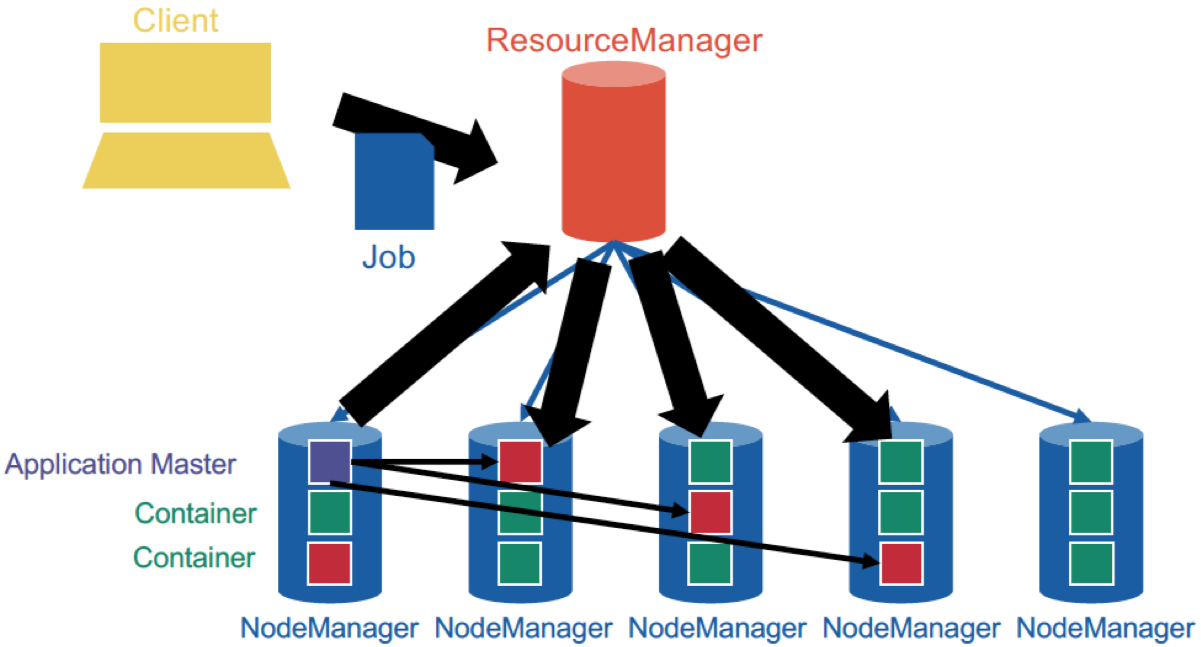
\includegraphics[width=0.7\textwidth]{Figures/YARNArchitecture.png}
    \caption{YARN Architecture}\label{fig:YARNArch}
\end{figure}

Thus, YARN cleanly separates between the general management of resources and bootstrapping new applications, which remains centralized on the coordinator node, and monitoring the job lifecycle, which is now delegated to one or more ApplicationMasters running concurrently. This means, in particular, that several applications can run concurrently in the same cluster.

\subsubsection{Resource Management}
There are four specific resources used in a distributed database system: Memory, CPU, Disk I/O and Network I/O. Most resource management systems (e.g. YARN) focus mainly on allocating and sharing memory and CPU.

ApplicationMasters can request and release containers at any time, dynamically. A container request is typically made by the ApplicationMasters with a specific demand. If the request is granted by the ResourceManager fully or partially, this is done indirectly by signing and issuing a container token to the ApplicationMaster that acts as proof that the resource was granted.

The ApplicationMaster can then connect to the allocated NodeManager and send the token. The NodeManager will then check the validity of the token and provide the memory and CPU granted by the ResourceManager. The ApplicationMaster ships the code (e.g., as a jar file) as well as parameters, which then runs as a process with exclusive use of this memory and CPU.

To bootstrap a new application, the ResourceManager can also issue application tokens to external clients so they can start the Application- Master.

There are as many ApplicationMasters as jobs. But only one resource manager. The ResourceManager does not monitor tasks and it does not restart upon failure.

The ApplicationMaster is application-specific. YARN is fully agnostic about the technology you are using.

\subsubsection{Job Lifecycle Management and Fault Tolerance}

The ApplicationMaster requests containers for the Map phase, and sets these containers up to execute Map tasks. As soon as a container is done executing a Map task, the ApplicationMaster will assign a new Map task to this container from the remaining queue, until no Map tasks are left.

It's the job of the ApplicationMaster to monitor for a failed task, and relaunch it with another container.


\subsection{Scheduling Stragegies}

\subsubsection{FIFO Scheduling}
In FIFO (First In First Out) scheduling, there is one application at a time running on the entire cluster. When it is done, the next application runs again on the entire cluster, and so on.

\subsubsection{Capacity Scheduling}
In capacity scheduling, the resources of the cluster are partitioned into several sub-clusters of various sizes. Each one of these sub-clusters has its own queue of applications running in a FIFO fashion within this queue.

Capacity scheduling also exists in a more "dynamic flavour" in which, when a sub-cluster is not currently used, its resources can be temporarily lent to the other sub-clusters. This is also in the spirit of usage maximization, so that the company as a whole will not waste unused resources.

\subsubsection{Fair Scheduling}
Fair scheduling involves more complex algorithms that attempt to allocate resources in a way fair to all users of the cluster and based on the share they are normally entitled to.

Fair scheduling should be understood in a dynamic fashion: the cluster has, at any point in time, users from various departments running their applications. Applications are dynamically and regularly requesting many containers with specific memory and CPU requirements, and releasing them again. Thus, fair scheduling consists on making dynamic decisions regarding which requests get granted and which requests have to wait.

\textcolor{grey}{More detail on Fair Scheduling in the Script on pages 268 and 289.}


\subsection{Summary}
\begin{itemize}
    \item We separate between scheduling and monitoring. (Scheduling is done by the ResourceManager and monitoring is done by the ApplicationMaster.)
    \item It is scalable. We can process more data than with the first version of map reduce.
    \item It is well available. You don't block the cluster unnecessarily. You don't have the bottleneck of the JobTracker anymore.
    \item It is multi-tenent. Meaning: you can have many people using the same cluster at the same time.
\end{itemize}
